\documentclass[11pt]{beamer}
\usepackage{booktabs,siunitx}
\usepackage{tikz}
\usepackage[compat=1.1.0]{tikz-feynman}
\usepackage[default]{opensans}
\usepackage[version=4]{mhchem}
\usetheme{Madrid}
\usefonttheme{default}
\useinnertheme{circles}
\sisetup{detect-all}
\setbeamertemplate{navigation symbols}{} % Uncomment this line to remove the navigation symbols from the bottom of all slides

\title[Charged Lepton Flavour Violation]{Charged Lepton Flavour Violation: \\ An Introduction to Muon Experiments} % The short title in the optional parameter appears at the bottom of every slide, the full title in the main parameter is only on the title page

% \subtitle{Optional Subtitle} % Presentation subtitle, remove this command if a subtitle isn't required

\author[Miles Kidson]{Miles Kidson} % Presenter name(s), the optional parameter can contain a shortened version to appear on the bottom of every slide, while the main parameter will appear on the title slide

\institute[UCT]{University of Cape Town \\ \smallskip \textit{kdsmil001@myuct.ac.za}} % Your institution, the optional parameter can be used for the institution shorthand and will appear on the bottom of every slide after author names, while the required parameter is used on the title slide and can include your email address or additional information on separate lines

\date[November 2022]{November 2022} % Presentation date or conference/meeting name, the optional parameter can contain a shortened version to appear on the bottom of every slide, while the required parameter value is output to the title slide

% \useoutertheme[subsection=false]{miniframes}

\begin{document}

\frame[plain]{\titlepage}

\begin{frame}
    \frametitle{Standard Model conserved quantities}
    \begin{columns}[c]
        \begin{column}{0.6\textwidth}
            There are a few quantities that are strictly conserved in SM processes:
            \bigskip
            \begin{itemize}
                \item Electric \& colour charge
                \item Baryon number $B$
                \item Lepton number $L$
            \end{itemize}
            \bigskip
            If neutrinos were massless, individual lepton flavour numbers $L_e$, $L_\mu$, and $L_\tau$ would be conserved\footnote[frame]{M.E. Peskin, 2018, p.286}. With massive neutrinos, only $L$ is conserved.

            (Provided neutrinos are Dirac fermions and not Majorana fermions)

        \end{column}
        \begin{column}{0.4\textwidth}
            \begin{figure}[h]
                \begin{center}
                    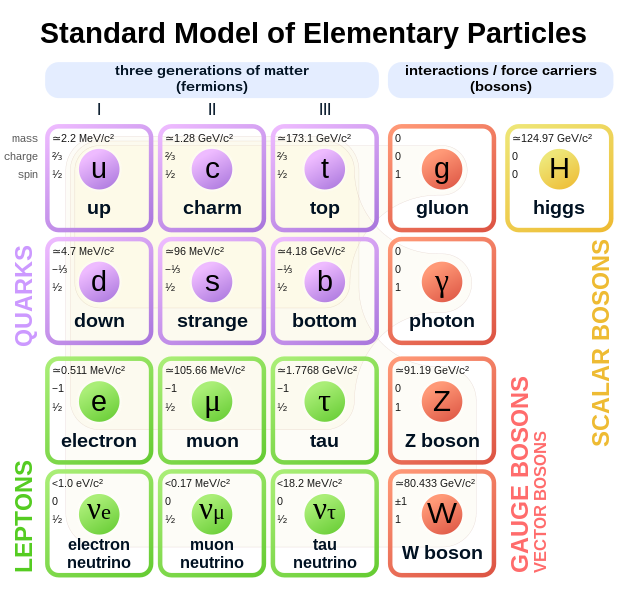
\includegraphics[width=\textwidth]{SM.png}
                \end{center}
            \end{figure}
            
        \end{column}
        
    \end{columns}

    

\end{frame}

\begin{frame}
    \frametitle{Charged Lepton Flavour Violation (CLFV)}
    \begin{columns}[c]
        \begin{column}{0.6\textwidth}
            \begin{itemize}
                \item We already see lepton flavour being violated in neutrino oscillation
                \item Best estimates of $\mu \rightarrow e\gamma$ rates by the same mechanism are $<$\num{e-54}, which are not realistically measurable\footnote[frame]{de Gouvea, A., \& Vogel, P. (2013). Lepton Flavor and Number Conservation, and Physics Beyond the Standard Model.}. Similar for other processes
                \item Thus observing these processes implies new physics is at play!
                \item Example processes would be $\mu\rightarrow e\,e\,e$, $\mu \rightarrow e\gamma$, and $\tau \rightarrow \mu,e + X$
                \item Muons are much easier to study than tau leptons
            \end{itemize}
        \end{column}

        \begin{column}{0.4\textwidth}
            \begin{tikzpicture}
                \begin{feynman}
                    \vertex (a);
                    \vertex [right=1.5cm of a] (b);
                    \vertex [right=1.5cm of b] (c);
                    \vertex [right=1.5cm of c] (d);
                    \vertex [above right=1.2cm of b] (b1);
                    \vertex [above right=1.5cm of b1] (b2);

                    \diagram {
                        (a) -- [fermion, edge label'=$\mu$] (b) -- [fermion, edge label'=$\nu_i$] (c) -- [fermion, edge label'=$e$] (d);
                        (b) -- [boson, quarter left, edge label=$W$] (b1) -- [boson, quarter left] (c);
                        (b1) -- [photon, edge label=$\gamma$] (b2);
                    };

                \end{feynman}
            \end{tikzpicture}
        \end{column}
    \end{columns}
\end{frame}

\begin{frame}
    \frametitle{$\mu\rightarrow e\,e\,e$}
    \begin{columns}[c]
        \begin{column}{0.6\textwidth}
            \begin{itemize}
                \item We could see this as $\mu^+\rightarrow e^+ e^+ e^- \nu_\mu \overline{\nu}_e$ and not be new physics
                \item Thus we look for this with no missing energy
                \item Could be $\mu \rightarrow e\gamma$ with more steps, or could be something else entirely
                \item The SINDRUM experiment put a rate limit of \num{e-12} with future experiments (Mu3e) aiming for \num{e-16}.\footnote[frame]{Ardu, M., \& Pezzullo, G. (2022). Introduction to Charged Lepton Flavour Violation}
            \end{itemize}
        \end{column}

        \begin{column}{0.4\textwidth}
            \begin{tikzpicture}
                \begin{feynman}
                    \vertex (a);
                    \vertex [right=1.5cm of a, blob] (b) {};
                    \vertex [right=1.5cm of b] (c);
                    % \vertex [right=1.5cm of c] (d);
                    % \vertex [above right=1.2cm of b] (b1);
                    \vertex [above right=1.5cm of b] (b2);
                    \vertex [above right=0.7cm of b2] (b3) {$e^-$};
                    \vertex [below right=0.7cm of b2] (b4) {$e^+$};


                    \diagram {
                        (b) -- [fermion, edge label=$\mu^+$] (a);
                        (c) -- [fermion, edge label=$e^+$] (b);
                        %  -- [fermion, edge label=$\overline{\nu}_i$] 
                        % (b) -- [plain, quarter left] (b1) -- [plain, quarter left] (c);
                        % (b) -- [plain, half right] (c);
                        (b) -- [photon, edge label=$\gamma$] (b2);
                        (b2) -- [fermion] (b3);
                        (b4) -- [fermion] (b2);
                    };

                \end{feynman}
            \end{tikzpicture}
            \bigskip

            \begin{tikzpicture}
                \begin{feynman}
                    \vertex (a);
                    \vertex [right=1.5cm of a, blob] (b);
                    \vertex [above right=1.5cm of b] (c);
                    \vertex [below right=1.5cm of b] (d);
                    \vertex [above right=1.5cm of c] (e) {$e^+$};
                    \vertex [below right=1.5cm of c] (f) {$e^-$};

                    \diagram {
                        (b) -- [fermion, edge label=$\mu^+$] (a);
                        (d) -- [fermion, edge label=$e^+$] (b);
                        (b) -- [ghost, edge label=?] (c);
                        (e) -- [fermion] (c);
                        (c) -- [fermion] (f);

                    };
                \end{feynman}
            \end{tikzpicture}
        \end{column}
    \end{columns}
\end{frame}

% \begin{itemize}
%     \item $\mu\rightarrow e\,e\,e$
%     \item $\mu N \rightarrow e N$
%     \item $\mu \rightarrow e\gamma$: $<\num{4.2e-13}$ at 90\% CL
% \end{itemize}

\begin{frame}
    \frametitle{$\mu^- N \rightarrow e^- N$}

    \begin{columns}[c]
        \begin{column}{0.6\textwidth}
            \begin{itemize}
                \item Conversion of a muon captured by a nucleus into an electron
                \item Bombarding nuclei with muons to see an outgoing electron
                \item Should result in a monoenergetic electron, $\approx$\SI{105}{\mega\electronvolt} for most nuclei
                \item Important to ignore $\mu^-\rightarrow e^- \overline{\nu}_e \nu_\mu$
                \item Rates for gold and titanium are $\lesssim$ \num{e-13} from SINDRUM-II\footnote[frame]{Bertl, W., Engfer, R., Hermes, E. et al. A search for $\mu$-e conversion in muonic gold. (2006)}
                \item Has potential to get to \num{e-18} at Fermilab and J-PARC with Al target
            \end{itemize}
        \end{column}
        \begin{column}{0.4\textwidth}
            \begin{figure}[h]
                \begin{center}
                    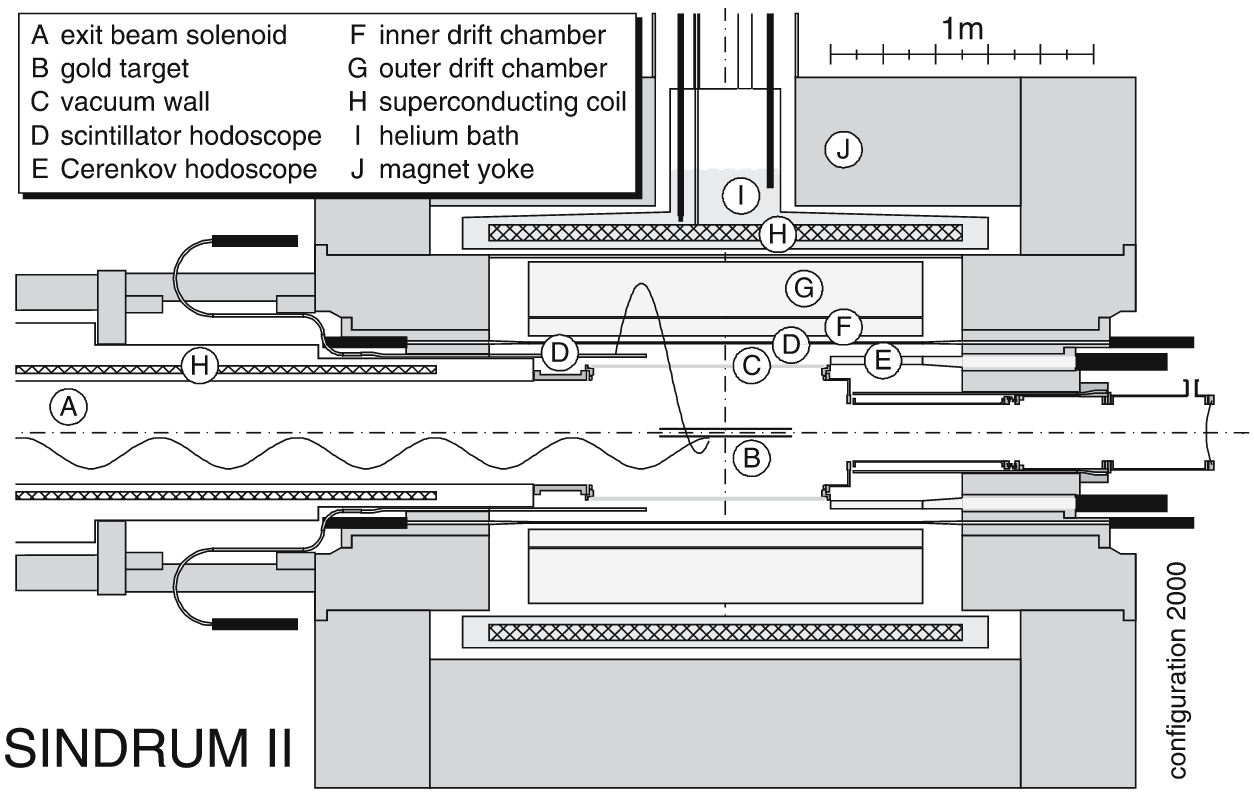
\includegraphics[width=\textwidth]{SINDRUMII.png}
                \end{center}
            \end{figure}
        \end{column}
    \end{columns}
    

\end{frame}

\begin{frame}
    \frametitle{$\mu^+ \rightarrow e^+ \gamma$}
    \begin{columns}[c]
        \begin{column}{0.6\textwidth}
            \begin{itemize}
                \item Longest studied process and with the most potential to reduce limits
                \item Background events are $\mu^+ \rightarrow e^+ \overline{\nu}_e \nu_\mu$ 
                \item Must look for total energy of $e +\gamma$ to be $m_\mu$
                \item MEG experiment reduced limits to \num{4.2e-13} in 2016\footnote[frame]{Meucci, M. (2022). MEG II experiment status and prospect.}
            \end{itemize}
        \end{column}

        \begin{column}{0.4\textwidth}
            \begin{tikzpicture}
                \begin{feynman}
                    \vertex (a) {$\mu^+$};
                    \vertex [right=of a,blob](b) {};
                    \vertex [right=of b] (c) {$e^+$};
                    \vertex [above right=2cm of b] (d) {$\gamma$};

                    % \vertex [left=of b] (a);
                    % \vertex [right=of b] (c);
                    % \vertex [above right=of b] (c);
                    % \vertex [below right=of b] (d);

                    \diagram{
                        (b) -- [fermion] (a),
                        (c) -- [fermion] (b),
                        (b) -- [photon] (d);
                        % (b) -- [fermion] (d);
                    };
                \end{feynman}
            \end{tikzpicture}
            
        \end{column}
    \end{columns}
    

\end{frame}

\begin{frame}
    \frametitle{What the heck is MEG?}
    \begin{columns}[t]
        \begin{column}{0.4\textwidth}
            \begin{itemize}
                \item Muon Electron Gamma detector at PSI in Zurich
                \item \num{3e7} $\mu^+$ per second beam incident onto polyethylene stopping target
                \item Looks for coincident $e^+$ and $\gamma$ events, each with energy \SI{52.8}{\mega\electronvolt}
                \item MEG-II {\footnotesize(Electric Boogaloo)} aims to bring the limit down to \num{6e-14}
            \end{itemize}
        \end{column}
    
        \begin{column}{0.6\textwidth}
            \begin{itemize}
                \item Large scintillation detector for photons and a drift chamber for positron spectrometry
            \end{itemize}
            \begin{figure}[h]
                \begin{center}
                    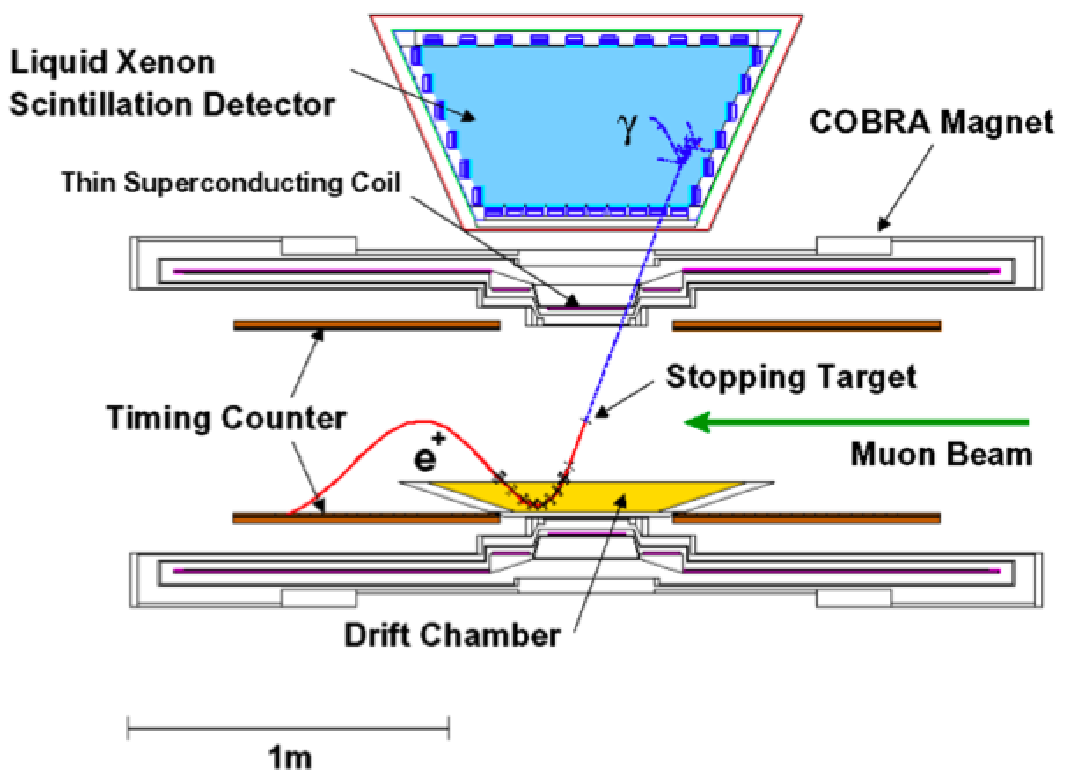
\includegraphics[width=.8\textwidth]{MEG.png}
                \end{center}
            \end{figure}
            
        \end{column}
    \end{columns}

    

\end{frame}

\begin{frame}
    \frametitle{Conclusion}
    \begin{itemize}
        \item CLFV is allowed in the SM, but with rates far too low to be detected
        \item Seeing CLFV implies new physics is at play and could also help explain neutrino mass and oscillation
        \item Muon processes are most commonly studied, with upper limits on rates nearing \num{e-14} in some cases
        \item The new MEG-II detector and Al target muon conversion experiments show promise to greatly reduce those limits
    \end{itemize}
    

\end{frame}

\begin{frame}[allowframebreaks]{References} 
    \nocite{*}
    \bibliographystyle{unsrt}
    \bibliography{bibliography}
\end{frame}


\end{document}